%%%---PREAMBLE---%%%%%%%%%%%%%%%%%%%%%%%%%%%%
\documentclass[twoside,12pt,final]{ucthesis-CA2012}

% fix for pandoc 1.14
\providecommand{\tightlist}{%
  \setlength{\itemsep}{0pt}\setlength{\parskip}{0pt}}

%--- Packages ---------------------------------------------------------
\usepackage[lofdepth,lotdepth,caption=false]{subfig}
\usepackage{fancyhdr}
\usepackage{amsmath, amssymb, graphicx}
\usepackage{xspace}
\usepackage{braket}
\usepackage{color}
\usepackage{setspace}
\usepackage{fancyvrb}
\usepackage{array}
\usepackage{ifxetex,ifluatex}
\usepackage{etoolbox}
\usepackage{booktabs}
\usepackage{xcolor}
\usepackage{tabu}
\usepackage{longtable}
\usepackage{titlesec}
%---New Definitions and Commands------------------------------------------------------

\newtheorem{theorem}{Jibberish}

\bibliography{references}

\hyphenation{mar-gin-al-ia}

% from uw_template.tex

% commands and environments needed by pandoc snippets
% extracted from the output of `pandoc -s`
%% Make R markdown code chunks work

\ifxetex
  \usepackage{fontspec,xltxtra,xunicode}
  \defaultfontfeatures{Mapping=tex-text,Scale=MatchLowercase}
\else
  \ifluatex
    \usepackage{fontspec}
    \defaultfontfeatures{Mapping=tex-text,Scale=MatchLowercase}
  \else
    \usepackage[utf8]{inputenc}
  \fi
\fi
\DefineShortVerb[commandchars=\\\{\}]{\|}
\DefineVerbatimEnvironment{Highlighting}{Verbatim}{commandchars=\\\{\}}
% Add ',fontsize=\small' for more characters per line
\newenvironment{Shaded}{}{}
\newcommand{\KeywordTok}[1]{\textcolor[rgb]{0.00,0.44,0.13}{\textbf{{#1}}}}
\newcommand{\DataTypeTok}[1]{\textcolor[rgb]{0.56,0.13,0.00}{{#1}}}
\newcommand{\DecValTok}[1]{\textcolor[rgb]{0.25,0.63,0.44}{{#1}}}
\newcommand{\BaseNTok}[1]{\textcolor[rgb]{0.25,0.63,0.44}{{#1}}}
\newcommand{\FloatTok}[1]{\textcolor[rgb]{0.25,0.63,0.44}{{#1}}}
\newcommand{\CharTok}[1]{\textcolor[rgb]{0.25,0.44,0.63}{{#1}}}
\newcommand{\StringTok}[1]{\textcolor[rgb]{0.25,0.44,0.63}{{#1}}}
\newcommand{\CommentTok}[1]{\textcolor[rgb]{0.38,0.63,0.69}{\textit{{#1}}}}
\newcommand{\OtherTok}[1]{\textcolor[rgb]{0.00,0.44,0.13}{{#1}}}
\newcommand{\AlertTok}[1]{\textcolor[rgb]{1.00,0.00,0.00}{\textbf{{#1}}}}
\newcommand{\FunctionTok}[1]{\textcolor[rgb]{0.02,0.16,0.49}{{#1}}}
\newcommand{\RegionMarkerTok}[1]{{#1}}
\newcommand{\ErrorTok}[1]{\textcolor[rgb]{1.00,0.00,0.00}{\textbf{{#1}}}}
\newcommand{\NormalTok}[1]{{#1}}
\newcommand{\OperatorTok}[1]{\textcolor[rgb]{0.00,0.44,0.13}{\textbf{{#1}}}}
\newcommand{\BuiltInTok}[1]{\textcolor[rgb]{0.00,0.44,0.13}{\textbf{{#1}}}}
\newcommand{\ControlFlowTok}[1]{\textcolor[rgb]{0.00,0.44,0.13}{\textbf{{#1}}}}

\newlength{\cslhangindent}
\setlength{\cslhangindent}{1.5em}
\newenvironment{cslreferences}%
{\setlength{\parindent}{0pt}%
\everypar{\setlength{\hangindent}{\cslhangindent}}\ignorespaces}%
{\par}

\ifxetex
  \usepackage[setpagesize=false, % page size defined by xetex
              unicode=false, % unicode breaks when used with xetex
              xetex,
              colorlinks=true,
              linkcolor=blue]{hyperref}
\else
  \usepackage[unicode=true,
              colorlinks=true,
              linkcolor=blue]{hyperref}
\fi
\hypersetup{breaklinks=true, pdfborder={0 0 0}}
\setlength{\parindent}{0pt}
\setlength{\parskip}{6pt plus 2pt minus 1pt}
\setlength{\emergencystretch}{3em}  % prevent overfull lines
\setcounter{secnumdepth}{0}

%---Set Margins ------------------------------------------------------
\setlength\oddsidemargin{0.25 in} \setlength\evensidemargin{0.25 in} \setlength\textwidth{6.25 in} \setlength\textheight{8.50 in}
\setlength\footskip{0.25 in} \setlength\topmargin{0 in} \setlength\headheight{0.25 in} \setlength\headsep{0.25 in}

%%%---DOCUMENT---%%%%%%%%%%%%%%%%%%%%%%%%%%%%
\begin{document}

%=== Preliminary Pages ============================================
\begin{ucfrontmatter}

  %%%%%%%%%%%%%%%%%%%%%%%%%%%
  % TITLE PAGE INFORMATION %
  %%%%%%%%%%%%%%%%%%%%%%%%%%%

  \title{Improving the Management of Marine Resources through Economics and Data Science}

  \author{Daniel A. Ovando}

  \report{Dissertation} \degree{Doctor of Philosophy} \degreemonth{June} \degreeyear{2018}
  \defensemonth{May}
  \defenseyear{2018}

  \chair{Professor Christopher Costello}  % this is your advisor
  \othermemberA{Professor Steven Gaines} % This is a member of your committee
  \othermemberB{Professor Ray Hilborn} % This is a member of your committee
  \othermemberC{Professor Olivier Deschenes} % This is a member of your committee (if your department requires 4 members)
  \numberofmembers{4} % should match the number of entries above (chair + othermembers)

  \field{Slowly and Painfully Working Out the Surprisingly Obvious}
  \campus{Santa Barbara}
	\maketitle
	\approvalpage
	\copyrightpage

  %%%%%%%%%%%%%%%%%%%%%%%%%%%
  % DEDICATION PAGE INFORMATION %
  %%%%%%%%%%%%%%%%%%%%%%%%%%%
    \begin{dedication}

      \vspace*{25ex}
      \begin{center}
      \begin{Large}

        To Hobbes

      \end{Large}
      \end{center}
  \end{dedication}
  \begin{acknowledgements}
    Thanks everyone!
  \end{acknowledgements}
  %%%%%%
  % CV %
  %%%%%%
  \begin{vitae}
    \addcontentsline{toc}{chapter}{Curriculum Vitae}
    \begin{vitaesection}{Education}
    \vspace{-0.1cm}
    \item [2018]	Ph.D. in Environmental Science and Management (Expected), University of California, Santa Barbara.
    \item [2010]	MESM in in Environmental Science and Management, University of California, Santa Barbara.
    \item [2007]	B.S. in Ecosystem Science and Policy and Biology, University of Miami
    \end{vitaesection}
    \textbf{Publications}

    Anderson, S.C., Cooper, A.B., Jensen, O.P., Minto, C., Thorson, J.T., Walsh, J.C., Afflerbach, J., Dickey‐Collas, M., Kleisner, K.M., Longo, C., Osio, G.C., Ovando, D., Mosqueira, I., Rosenberg, A.A., Selig, E.R., n.d. Improving estimates of population status and trend with superensemble models. Fish and Fisheries 18, 732–741. https://doi.org/10.1111/faf.12200

 Burgess, M.G., McDermott, G.R., Owashi, B., Reeves, L.E.P., Clavelle, T., Ovando, D., Wallace, B.P., Lewison, R.L., Gaines, S.D., Costello, C., 2018. Protecting marine mammals, turtles, and birds by rebuilding global fisheries. Science 359, 1255–1258. https://doi.org/10.1126/science.aao4248

Costello, C., Ovando, D., Clavelle, T., Strauss, C.K., Hilborn, R., Melnychuk, M.C., Branch, T.A., Gaines, S.D., Szuwalski, C.S., Cabral, R.B., Rader, D.N., Leland, A., 2016. Global fishery prospects under contrasting management regimes. PNAS 113, 5125–5129. https://doi.org/10.1073/pnas.1520420113

Costello, C., Ovando, D., Hilborn, R., Gaines, S.D., Deschenes, O., Lester, S.E., 2012. Status and Solutions for the World’s Unassessed Fisheries. Science 338, 517–520. https://doi.org/10.1126/science.1223389

Dowling, N., Wilson, J., Rudd, M., Babcock, E., Caillaux, M., Cope, J., Dougherty, D., Fujita, R., Gedamke, T., Gleason, M., Guttierrez, M., Hordyk, A., Maina, G., Mous, P., Ovando, D., Parma, A., Prince, J., Revenga, C., Rude, J., Szuwalski, C., Valencia, S., Victor, S., 2016. FishPath: A Decision Support System for Assessing and Managing Data- and Capacity- Limited Fisheries, in: Quinn II, T., Armstrong, J., Baker, M., Heifetz, J., Witherell, D. (Eds.), Assessing and Managing Data-Limited Fish Stocks. Alaska Sea Grant, University of Alaska Fairbansk.

Fogarty, M.J., Rosenberg, A.A., Cooper, A.B., Dickey-Collas, M., Fulton, E.A., Gutiérrez, N.L., Hyde, K.J.W., Kleisner, K.M., Kristiansen, T., Longo, C., Minte-Vera, C.V., Minto, C., Mosqueira, I., Osio, G.C., Ovando, D., Selig, E.R., Thorson, J.T., Ye, Y., 2016. Fishery production potential of large marine ecosystems: A prototype analysis. Environmental Development, SI:Ecosystem-based LME Mgt 17, Supplement 1, 211–219. https://doi.org/10.1016/j.envdev.2016.02.001

Hammerschlag, N., Ovando, D., Serafy, J.E., 2010. Seasonal diet and feeding habits of juvenile fishes foraging along a subtropical marine ecotone. Aquatic Biology 9, 279–290.
Hilborn, R., Ovando, D., 2014. Reflections on the success of traditional fisheries management. ICES J. Mar. Sci. 71, 1040–1046. https://doi.org/10.1093/icesjms/fsu034

Ovando, D., Dougherty, D., Wilson, J.R., 2016a. Market and design solutions to the short-term economic impacts of marine reserves. Fish Fish n/a-n/a. https://doi.org/10.1111/faf.12153

Ovando, D., Poon, S., Costello, C., 2016b. Opportunities and precautions for integrating cooperation and individual transferable quotas with territorial use rights in fisheries. Bulletin of Marine Science.

Ovando, D., Deacon, R.T., Lester, S.E., Costello, C., Van Leuvan, T., McIlwain, K., Strauss, K.C., Arbuckle, M., Fujita, R., Gelcich, S., Uchida, H., 2013. Conservation incentives and collective choices in cooperative fisheries. Marine Policy 37, 132–140. https://doi.org/10.1016/j.marpol.2012.03.012
Rahimi, S., Gaines, S.D., Gelcich, S., Deacon, R., Ovando, D., 2016. Factors driving the implementation of fishery reforms. Marine Policy 71, 222–228. https://doi.org/10.1016/j.marpol.2016.06.005

Rosenberg, A.A., Fogarty, M.J., Cooper, A.B., Dickey-Collas, M., Fulton, E.A., Gutiérrez, N.L., Hyde, K.J.W., Kleisner, K.M., Kristiansen, T., Longo, C., Minte-Vera, C., Minto, C., Mosqueira, I., Chato Osio, G., Ovando, D., Selig, E.R., Thorson, J.T., Ye, Y., 2014. Developing new approaches to global stock status assessment and fishery production potential of the seas, FAO Fisheries and Aquaculture Circular. Food and Agriculture Organization of the United Nations.

Rosenberg, A.A., Kleisner, K.M., Afflerbach, J., Anderson, S.C., Dickey-Collas, M., Cooper, A.B., Fogarty, M.J., Fulton, E.A., Gutiérrez, N.L., Hyde, K.J.W., Jardim, E., Jensen, O.P., Kristiansen, T., Longo, C., Minte-Vera, C.V., Minto, C., Mosqueira, I., Osio, G.C., Ovando, D., Selig, E.R., Thorson, J.T., Walsh, J.C., Ye, Y., 2017. Applying a New Ensemble Approach to Estimating Stock Status of Marine Fisheries around the World. CONSERVATION LETTERS n/a-n/a. https://doi.org/10.1111/conl.12363

Szuwalski, C.S., Castrejon, M., Ovando, D., Chasco, B., 2016. An integrated stock assessment for red spiny lobster (Panulirus penicillatus) from the Galapagos Marine Reserve. Fisheries Research 177, 82–94. https://doi.org/10.1016/j.fishres.2016.01.002


  \end{vitae}
	%%%%%%%%%%%%%%%%%%%%%%%%%%%
  % ABSTRACT %
  %%%%%%%%%%%%%%%%%%%%%%%%%%%
  \begin{abstract}
    \addcontentsline{toc}{chapter}{Abstract}
    %todo: max 350 words

    The data say `meh'

    %\abstractsignature
  \end{abstract}
	\tableofcontents

	  \listoftables
  
    \listoffigures
  
\end{ucfrontmatter}
\begin{ucmainmatter}

\hypertarget{ucsb-thesis-fields}{%
\chapter{UCSB thesis fields}\label{ucsb-thesis-fields}}

Placeholder

\hypertarget{intro}{%
\chapter{Introduction}\label{intro}}
\begin{Shaded}
\begin{Highlighting}[]
\KeywordTok{getwd}\NormalTok{()}
\end{Highlighting}
\end{Shaded}
\begin{verbatim}
[1] "D:/Projects_R/MasterThesis/index"
\end{verbatim}
test

Welcome to the \emph{R Markdown} thesis template. This template is based on (and in many places copied directly from) the UW LaTeX template, but hopefully it will provide a nicer interface for those that have never used TeX or LaTeX before. Using \emph{R Markdown} will also allow you to easily keep track of your analyses in \textbf{R} chunks of code, with the resulting plots and output included as well. The hope is this \emph{R Markdown} template gets you in the habit of doing reproducible research, which benefits you long-term as a researcher, but also will greatly help anyone that is trying to reproduce or build onto your results down the road.

Hopefully, you won't have much of a learning period to go through and you will reap the benefits of a nicely formatted thesis. The use of LaTeX in combination with \emph{Markdown} is more consistent than the output of a word processor, much less prone to corruption or crashing, and the resulting file is smaller than a Word file. While you may have never had problems using Word in the past, your thesis is likely going to be at least twice as large and complex as anything you've written before, taxing Word's capabilities. After working with \emph{Markdown} and \textbf{R} together for a few weeks, we are confident this will be your reporting style of choice going forward.

\textbf{Why use it?}

\emph{R Markdown} creates a simple and straightforward way to interface with the beauty of LaTeX. Packages have been written in \textbf{R} to work directly with LaTeX to produce nicely formatting tables and paragraphs. In addition to creating a user friendly interface to LaTeX, \emph{R Markdown} also allows you to read in your data, to analyze it and to visualize it using \textbf{R} functions, and also to provide the documentation and commentary on the results of your project. Further, it allows for \textbf{R} results to be passed inline to the commentary of your results. You'll see more on this later.

\textbf{Who should use it?}

Anyone who needs to use data analysis, math, tables, a lot of figures, complex cross-references, or who just cares about the final appearance of their document should use \emph{R Markdown}. Of particular use should be anyone in the sciences, but the user-friendly nature of \emph{Markdown} and its ability to keep track of and easily include figures, automatically generate a table of contents, index, references, table of figures, etc. should make it of great benefit to nearly anyone writing a thesis project.

\hypertarget{rmd-basics}{%
\chapter{R Markdown Basics}\label{rmd-basics}}

Placeholder

\hypertarget{lists}{%
\section{Lists}\label{lists}}

\hypertarget{line-breaks}{%
\section{Line breaks}\label{line-breaks}}

\hypertarget{r-chunks}{%
\section{R chunks}\label{r-chunks}}

\hypertarget{inline-code}{%
\section{Inline code}\label{inline-code}}

\hypertarget{including-plots}{%
\section{Including plots}\label{including-plots}}

\hypertarget{loading-and-exploring-data}{%
\section{Loading and exploring data}\label{loading-and-exploring-data}}

\hypertarget{additional-resources}{%
\section{Additional resources}\label{additional-resources}}

\hypertarget{math-sci}{%
\chapter{Mathematics and Science}\label{math-sci}}

Placeholder

\hypertarget{math}{%
\section{Math}\label{math}}

\hypertarget{chemistry-101-symbols}{%
\section{Chemistry 101: Symbols}\label{chemistry-101-symbols}}

\hypertarget{typesetting-reactions}{%
\subsection{Typesetting reactions}\label{typesetting-reactions}}

\hypertarget{other-examples-of-reactions}{%
\subsection{Other examples of reactions}\label{other-examples-of-reactions}}

\hypertarget{physics}{%
\section{Physics}\label{physics}}

\hypertarget{biology}{%
\section{Biology}\label{biology}}

\hypertarget{ref-labels}{%
\chapter{Results}\label{ref-labels}}

By far the easiest way to present tables in your thesis is to store the contents of the table in a CSV or Excel file, then read that file in to your R Markdown document as a data frame. Then you can style the table with the \texttt{kable} function, or functions in the \href{https://cran.r-project.org/web/packages/kableExtra/index.html}{kableExtra} pacakge.

In addition to the tables that can be automatically generated from a data frame in \textbf{R} that you saw in \protect\hyperlink{rmd-basics}{R Markdown Basics} using the \texttt{kable} function, you can also create tables using \emph{pandoc}. (More information is available at \url{http://pandoc.org/README.html\#tables}.) This might be useful if you don't have values specifically stored in \textbf{R}, but you'd like to display them in table form. Below is an example. Pay careful attention to the alignment in the table and hyphens to create the rows and columns. Generally I don't recommend this approach of typing the table directly into your R Markdown document.
\begin{longtable}[]{@{}ccc@{}}
\caption{\label{tab:inher} Correlation of Inheritance Factors for Parents and Child}\tabularnewline
\toprule
\begin{minipage}[b]{0.29\columnwidth}\centering
Factors\strut
\end{minipage} & \begin{minipage}[b]{0.46\columnwidth}\centering
Correlation between Parents \& Child\strut
\end{minipage} & \begin{minipage}[b]{0.16\columnwidth}\centering
Inherited\strut
\end{minipage}\tabularnewline
\midrule
\endfirsthead
\toprule
\begin{minipage}[b]{0.29\columnwidth}\centering
Factors\strut
\end{minipage} & \begin{minipage}[b]{0.46\columnwidth}\centering
Correlation between Parents \& Child\strut
\end{minipage} & \begin{minipage}[b]{0.16\columnwidth}\centering
Inherited\strut
\end{minipage}\tabularnewline
\midrule
\endhead
\begin{minipage}[t]{0.29\columnwidth}\centering
Education\strut
\end{minipage} & \begin{minipage}[t]{0.46\columnwidth}\centering
-0.49\strut
\end{minipage} & \begin{minipage}[t]{0.16\columnwidth}\centering
Yes\strut
\end{minipage}\tabularnewline
\begin{minipage}[t]{0.29\columnwidth}\centering
Socio-Economic Status\strut
\end{minipage} & \begin{minipage}[t]{0.46\columnwidth}\centering
0.28\strut
\end{minipage} & \begin{minipage}[t]{0.16\columnwidth}\centering
Slight\strut
\end{minipage}\tabularnewline
\begin{minipage}[t]{0.29\columnwidth}\centering
Income\strut
\end{minipage} & \begin{minipage}[t]{0.46\columnwidth}\centering
0.08\strut
\end{minipage} & \begin{minipage}[t]{0.16\columnwidth}\centering
No\strut
\end{minipage}\tabularnewline
\begin{minipage}[t]{0.29\columnwidth}\centering
Family Size\strut
\end{minipage} & \begin{minipage}[t]{0.46\columnwidth}\centering
0.18\strut
\end{minipage} & \begin{minipage}[t]{0.16\columnwidth}\centering
Slight\strut
\end{minipage}\tabularnewline
\begin{minipage}[t]{0.29\columnwidth}\centering
Occupational Prestige\strut
\end{minipage} & \begin{minipage}[t]{0.46\columnwidth}\centering
0.21\strut
\end{minipage} & \begin{minipage}[t]{0.16\columnwidth}\centering
Slight\strut
\end{minipage}\tabularnewline
\bottomrule
\end{longtable}
We can also create a link to the table by doing the following: Table \ref{tab:inher}. If you go back to \protect\hyperlink{loading-and-exploring-data}{Loading and exploring data} and look at the \texttt{kable} table, we can create a reference to this max delays table too: Table \ref{tab:maxdelays}. The addition of the \texttt{(\textbackslash{}\#tab:inher)} option to the end of the table caption allows us to then make a reference to Table \texttt{\textbackslash{}@ref(tab:label)}. Note that this reference could appear anywhere throughout the document after the table has appeared.

\clearpage

\hypertarget{figures}{%
\section{Figures}\label{figures}}

Test

In the \textbf{R} chunk below, we will load in a picture stored as \texttt{uw.png} in our main directory. We then give it the caption of ``UW logo'', the label of ``uwlogo'', and specify that this is a figure. Make note of the different \textbf{R} chunk options that are given in the R Markdown file (not shown in the knitted document).

Here is a reference to the UW logo: Figure \ref{fig:uwlogo}. Note the use of the \texttt{fig:} code here. By naming the \textbf{R} chunk that contains the figure, we can then reference that figure later as done in the first sentence here. We can also specify the caption for the figure via the R chunk option \texttt{fig.cap}.

\clearpage

Below we will investigate how to save the output of an \textbf{R} plot and label it in a way similar to that done above. Recall the \texttt{flights} dataset from Chapter \ref{rmd-basics}. (Note that we've shown a different way to reference a section or chapter here.) We will next explore a bar graph with the mean flight departure delays by airline from Portland for 2014. Note also the use of the \texttt{scale} parameter which is discussed on the next page.
\begin{Shaded}
\begin{Highlighting}[]
\NormalTok{flights }\OperatorTok\StringTok{ }\KeywordTok{group_by}\NormalTok{(carrier) }\OperatorTok
\StringTok{  }\KeywordTok{summarize}\NormalTok{(}\DataTypeTok{mean_dep_delay =} \KeywordTok{mean}\NormalTok{(dep_delay)) }\OperatorTok
\StringTok{  }\KeywordTok{ggplot}\NormalTok{(}\KeywordTok{aes}\NormalTok{(}\DataTypeTok{x =}\NormalTok{ carrier, }\DataTypeTok{y =}\NormalTok{ mean_dep_delay)) }\OperatorTok{+}
\StringTok{  }\KeywordTok{geom_bar}\NormalTok{(}\DataTypeTok{position =} \StringTok{"identity"}\NormalTok{, }\DataTypeTok{stat =} \StringTok{"identity"}\NormalTok{, }\DataTypeTok{fill =} \StringTok{"red"}\NormalTok{)}
\end{Highlighting}
\end{Shaded}
\begin{verbatim}
`summarise()` ungrouping output (override with `.groups` argument)
\end{verbatim}
\begin{figure}
\centering
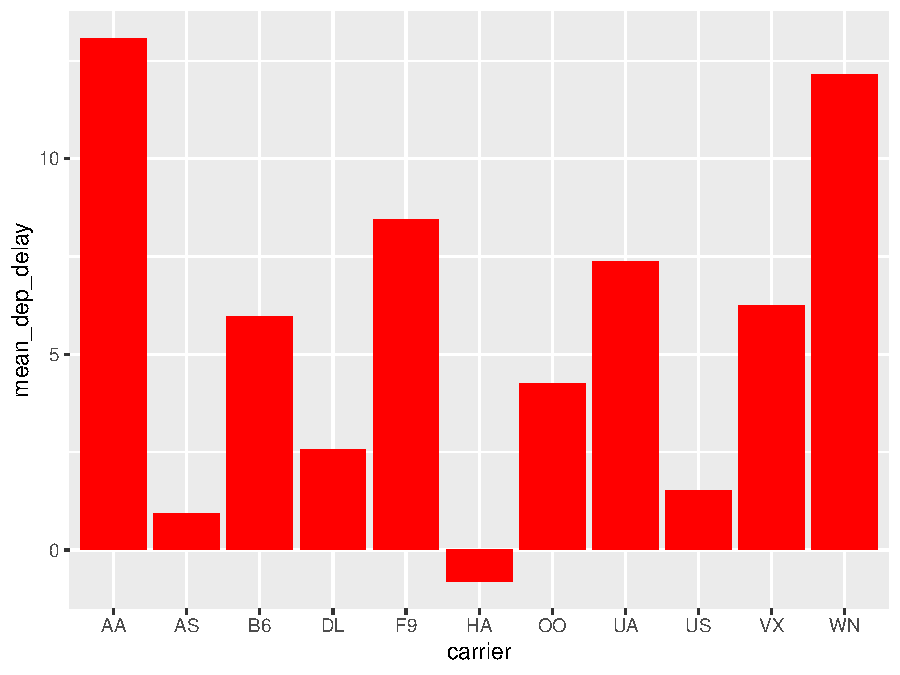
\includegraphics{thesis_files/figure-latex/delaysboxplot-1.pdf}
\caption{\label{fig:delaysboxplot}Mean Delays by Airline}
\end{figure}
Here is a reference to this image: Figure \ref{fig:delaysboxplot}.

A table linking these carrier codes to airline names is available at \url{https://github.com/ismayc/pnwflights14/blob/master/data/airlines.csv}.

\clearpage

Next, we will explore the use of the \texttt{out.extra} chunk option, which can be used to shrink or expand an image loaded from a file by specifying \texttt{"scale=\ "}. Here we use the mathematical graph stored in the ``subdivision.pdf'' file.

Here is a reference to this image: Figure \ref{fig:subd}. Note that \texttt{echo=FALSE} is specified so that the \textbf{R} code is hidden in the document.

\textbf{Knit Child}
\begin{figure}
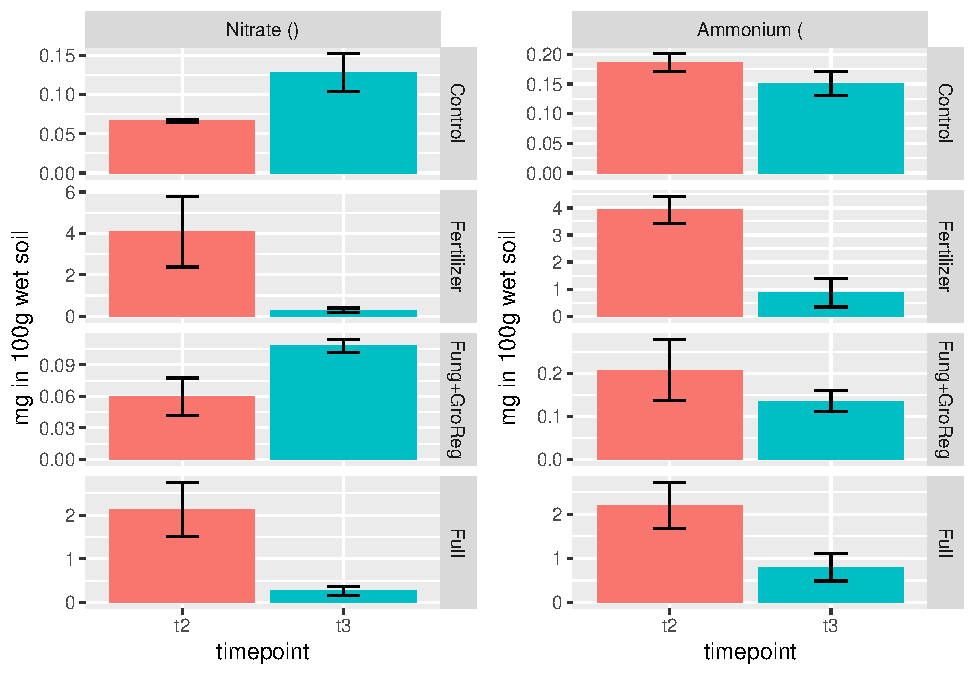
\includegraphics[scale=0.75]{thesis_files/figure-latex/subd-1} \caption{Subdiv. graph}\label{fig:subd}
\end{figure}
\hypertarget{footnotes-and-endnotes}{%
\section{Footnotes and Endnotes}\label{footnotes-and-endnotes}}

You might want to footnote something.\footnote{footnote text} The footnote will be in a smaller font and placed appropriately. Endnotes work in much the same way.

\hypertarget{bibliographies}{%
\section{Bibliographies}\label{bibliographies}}

Of course you will need to cite things, and you will probably accumulate an armful of sources. There are a variety of tools available for creating a bibliography database (stored with the .bib extension). In addition to BibTeX suggested below, you may want to consider using the free and easy-to-use tool called Zotero. Some Zotero documentation is at \url{http://libguides.reed.edu/citation/zotero}. In addition, a tutorial is available from Middlebury College at \url{http://sites.middlebury.edu/zoteromiddlebury/}.

\emph{R Markdown} uses \emph{pandoc} (\url{http://pandoc.org/}) to build its bibliographies. One nice caveat of this is that you won't have to do a second compile to load in references as standard LaTeX requires. To cite references in your thesis (after creating your bibliography database), place the reference name inside square brackets and precede it by the ``at'' symbol. For example, here's a reference to a book about worrying: {[}\protect\hyperlink{ref-Molina1994}{1}{]}. This \texttt{Molina1994} entry appears in a file called \texttt{thesis.bib} in the \texttt{bib} folder. This bibliography database file was created by a program called BibTeX. You can call this file something else if you like (look at the YAML header in the main .Rmd file) and, by default, is to placed in the \texttt{bib} folder.

For more information about BibTeX and bibliographies, see (\url{http://web.reed.edu/cis/help/latex/index.html})\footnote{\protect\hyperlink{ref-reedweb2007}{2}}. There are three pages on this topic: \emph{bibtex} (which talks about using BibTeX, at \url{http://web.reed.edu/cis/help/latex/bibtex.html}), \emph{bibtexstyles} (about how to find and use the bibliography style that best suits your needs, at \url{http://web.reed.edu/cis/help/latex/bibtexstyles.html}) and \emph{bibman} (which covers how to make and maintain a bibliography by hand, without BibTeX, at \url{http://web.reed.edu/cis/help/latex/bibman.html}). The last page will not be useful unless you have only a few sources.

If you look at the YAML header at the top of the main .Rmd file you can see that we can specify the style of the bibliography by referencing the appropriate csl file. You can download a variety of different style files at \url{https://www.zotero.org/styles}. Make sure to download the file into the csl folder.

\textbf{Tips for Bibliographies}
\begin{itemize}
\tightlist
\item
  Like with thesis formatting, the sooner you start compiling your bibliography for something as large as thesis, the better.
\item
  The cite key (a citation's label) needs to be unique from the other entries.
\item
  When you have more than one author or editor, you need to separate each author's name by the word ``and'' e.g.~\texttt{Author\ =\ \{Noble,\ Sam\ and\ Youngberg,\ Jessica\},}.
\item
  Bibliographies made using BibTeX (whether manually or using a manager) accept LaTeX markup, so you can italicize and add symbols as necessary.
\item
  To force capitalization in an article title or where all lowercase is generally used, bracket the capital letter in curly braces.
\end{itemize}
\hypertarget{anything-else}{%
\section{Anything else?}\label{anything-else}}

If you'd like to see examples of other things in this template, please \href{https://github.com/benmarwick/huskydown/issues/new}{contact us} (email \href{mailto:bmarwick@uw.edu}{\nolinkurl{bmarwick@uw.edu}}) with your suggestions. We love to see people using \emph{R Markdown} for their theses, and are happy to help.

\hypertarget{conclusion}{%
\chapter*{Conclusion}\label{conclusion}}
\addcontentsline{toc}{chapter}{Conclusion}

If we don't want Conclusion to have a chapter number next to it, we can add the \texttt{\{-\}} attribute.

\textbf{More info}

And here's some other random info: the first paragraph after a chapter title or section head \emph{shouldn't be} indented, because indents are to tell the reader that you're starting a new paragraph. Since that's obvious after a chapter or section title, proper typesetting doesn't add an indent there.

\appendix

\hypertarget{the-first-appendix}{%
\chapter{The First Appendix}\label{the-first-appendix}}

This first appendix includes all of the R chunks of code that were hidden throughout the document (using the \texttt{include\ =\ FALSE} chunk tag) to help with readibility and/or setup.

\textbf{In the main Rmd file}

\textbf{In Chapter \ref{ref-labels}:}
\begin{Shaded}
\begin{Highlighting}[]
\CommentTok{# This chunk ensures that the huskydown package is}
\CommentTok{# installed and loaded. This huskydown package includes}
\CommentTok{# the template files for the thesis and also two functions}
\CommentTok{# used for labeling and referencing}
\ControlFlowTok{if}\NormalTok{(}\OperatorTok{!}\KeywordTok{require}\NormalTok{(devtools))}
  \KeywordTok{install.packages}\NormalTok{(}\StringTok{"devtools"}\NormalTok{, }\DataTypeTok{repos =} \StringTok{"http://cran.rstudio.com"}\NormalTok{)}
\ControlFlowTok{if}\NormalTok{(}\OperatorTok{!}\KeywordTok{require}\NormalTok{(dplyr))}
    \KeywordTok{install.packages}\NormalTok{(}\StringTok{"dplyr"}\NormalTok{, }\DataTypeTok{repos =} \StringTok{"http://cran.rstudio.com"}\NormalTok{)}
\ControlFlowTok{if}\NormalTok{(}\OperatorTok{!}\KeywordTok{require}\NormalTok{(ggplot2))}
    \KeywordTok{install.packages}\NormalTok{(}\StringTok{"ggplot2"}\NormalTok{, }\DataTypeTok{repos =} \StringTok{"http://cran.rstudio.com"}\NormalTok{)}
\ControlFlowTok{if}\NormalTok{(}\OperatorTok{!}\KeywordTok{require}\NormalTok{(ggplot2))}
    \KeywordTok{install.packages}\NormalTok{(}\StringTok{"bookdown"}\NormalTok{, }\DataTypeTok{repos =} \StringTok{"http://cran.rstudio.com"}\NormalTok{)}
\ControlFlowTok{if}\NormalTok{(}\OperatorTok{!}\KeywordTok{require}\NormalTok{(gauchodown))\{}
  \KeywordTok{library}\NormalTok{(devtools)}
\NormalTok{  devtools}\OperatorTok{::}\KeywordTok{install_github}\NormalTok{(}\StringTok{"benmarwick/gauchodown"}\NormalTok{)}
\NormalTok{  \}}
\KeywordTok{library}\NormalTok{(gauchodown)}
\NormalTok{flights <-}\StringTok{ }\KeywordTok{read.csv}\NormalTok{(}\StringTok{"data/flights.csv"}\NormalTok{)}
\end{Highlighting}
\end{Shaded}
\hypertarget{the-second-appendix-for-fun}{%
\chapter{The Second Appendix, for Fun}\label{the-second-appendix-for-fun}}

\hypertarget{colophon}{%
\chapter*{Colophon}\label{colophon}}
\addcontentsline{toc}{chapter}{Colophon}

This document is set in \href{https://github.com/georgd/EB-Garamond}{EB Garamond}, \href{https://github.com/adobe-fonts/source-code-pro/}{Source Code Pro} and \href{http://www.latofonts.com/lato-free-fonts/}{Lato}. The body text is set at 11pt with \(\familydefault\).

It was written in R Markdown and \(\LaTeX\), and rendered into PDF using \href{https://github.com/danovando/gauchodown}{gauchodown} and \href{https://github.com/rstudio/bookdown}{bookdown}.

This document was typeset using the XeTeX typesetting system, and the \href{http://staff.washington.edu/fox/tex/}{University of Washington Thesis class} class created by Jim Fox. Under the hood, the \href{https://github.com/UWIT-IAM/UWThesis}{University of Washington Thesis LaTeX template} is used to ensure that documents conform precisely to submission standards. Other elements of the document formatting source code have been taken from the \href{https://github.com/stevenpollack/ucbthesis}{Latex, Knitr, and RMarkdown templates for UC Berkeley's graduate thesis}, and \href{https://github.com/suchow/Dissertate}{Dissertate: a LaTeX dissertation template to support the production and typesetting of a PhD dissertation at Harvard, Princeton, and NYU}

The source files for this thesis, along with all the data files, have been organised into an R package, xxx, which is available at \url{https://github.com/xxx/xxx}. A hard copy of the thesis can be found in the University of Washington library.

This version of the thesis was generated on 2021-01-11 16:32:36. The repository is currently at this commit:

The computational environment that was used to generate this version is as follows:
\begin{verbatim}
- Session info ---------------------------------------------------------------
 setting  value                       
 version  R version 4.0.3 (2020-10-10)
 os       Windows 10 x64              
 system   x86_64, mingw32             
 ui       RTerm                       
 language (EN)                        
 collate  English_United States.1252  
 ctype    English_United States.1252  
 tz       Europe/Berlin               
 date     2021-01-11                  

- Packages -------------------------------------------------------------------
 package     * version date       lib source                               
 abind         1.4-5   2016-07-21 [1] CRAN (R 4.0.3)                       
 assertthat    0.2.1   2019-03-21 [1] CRAN (R 4.0.3)                       
 backports     1.2.0   2020-11-02 [1] CRAN (R 4.0.3)                       
 bookdown      0.21.6  2021-01-11 [1] Github (rstudio/bookdown@92c59d3)    
 broom         0.7.3   2020-12-16 [1] CRAN (R 4.0.3)                       
 callr         3.5.1   2020-10-13 [1] CRAN (R 4.0.3)                       
 car           3.0-10  2020-09-29 [1] CRAN (R 4.0.3)                       
 carData       3.0-4   2020-05-22 [1] CRAN (R 4.0.3)                       
 cellranger    1.1.0   2016-07-27 [1] CRAN (R 4.0.3)                       
 cli           2.2.0   2020-11-20 [1] CRAN (R 4.0.3)                       
 colorspace    2.0-0   2020-11-11 [1] CRAN (R 4.0.3)                       
 cowplot       1.1.1   2020-12-30 [1] CRAN (R 4.0.3)                       
 crayon        1.3.4   2017-09-16 [1] CRAN (R 4.0.3)                       
 curl          4.3     2019-12-02 [1] CRAN (R 4.0.3)                       
 data.table    1.13.4  2020-12-08 [1] CRAN (R 4.0.3)                       
 DBI           1.1.0   2019-12-15 [1] CRAN (R 4.0.3)                       
 dbplyr        2.0.0   2020-11-03 [1] CRAN (R 4.0.3)                       
 desc          1.2.0   2018-05-01 [1] CRAN (R 4.0.3)                       
 devtools    * 2.3.2   2020-09-18 [1] CRAN (R 4.0.3)                       
 digest        0.6.27  2020-10-24 [1] CRAN (R 4.0.3)                       
 dplyr       * 1.0.2   2020-08-18 [1] CRAN (R 4.0.3)                       
 ellipsis      0.3.1   2020-05-15 [1] CRAN (R 4.0.3)                       
 evaluate      0.14    2019-05-28 [1] CRAN (R 4.0.3)                       
 fansi         0.4.1   2020-01-08 [1] CRAN (R 4.0.3)                       
 farver        2.0.3   2020-01-16 [1] CRAN (R 4.0.3)                       
 forcats     * 0.5.0   2020-03-01 [1] CRAN (R 4.0.3)                       
 foreign       0.8-80  2020-05-24 [2] CRAN (R 4.0.3)                       
 fs            1.5.0   2020-07-31 [1] CRAN (R 4.0.3)                       
 gauchodown  * 1.0     2021-01-07 [1] Github (danovando/gauchodown@d9a19b8)
 generics      0.1.0   2020-10-31 [1] CRAN (R 4.0.3)                       
 ggplot2     * 3.3.3   2020-12-30 [1] CRAN (R 4.0.3)                       
 ggpubr      * 0.4.0   2020-06-27 [1] CRAN (R 4.0.3)                       
 ggsignif      0.6.0   2019-08-08 [1] CRAN (R 4.0.3)                       
 git2r         0.27.1  2020-05-03 [1] CRAN (R 4.0.3)                       
 glue          1.4.2   2020-08-27 [1] CRAN (R 4.0.3)                       
 gtable        0.3.0   2019-03-25 [1] CRAN (R 4.0.3)                       
 haven         2.3.1   2020-06-01 [1] CRAN (R 4.0.3)                       
 highr         0.8     2019-03-20 [1] CRAN (R 4.0.3)                       
 hms           0.5.3   2020-01-08 [1] CRAN (R 4.0.3)                       
 htmltools     0.5.0   2020-06-16 [1] CRAN (R 4.0.3)                       
 httr          1.4.2   2020-07-20 [1] CRAN (R 4.0.3)                       
 jsonlite      1.7.2   2020-12-09 [1] CRAN (R 4.0.3)                       
 knitr         1.30    2020-09-22 [1] CRAN (R 4.0.3)                       
 labeling      0.4.2   2020-10-20 [1] CRAN (R 4.0.3)                       
 lifecycle     0.2.0   2020-03-06 [1] CRAN (R 4.0.3)                       
 lubridate     1.7.9.2 2020-11-13 [1] CRAN (R 4.0.3)                       
 magrittr      2.0.1   2020-11-17 [1] CRAN (R 4.0.3)                       
 memoise       1.1.0   2017-04-21 [1] CRAN (R 4.0.3)                       
 modelr        0.1.8   2020-05-19 [1] CRAN (R 4.0.3)                       
 munsell       0.5.0   2018-06-12 [1] CRAN (R 4.0.3)                       
 openxlsx      4.2.3   2020-10-27 [1] CRAN (R 4.0.3)                       
 pillar        1.4.7   2020-11-20 [1] CRAN (R 4.0.3)                       
 pkgbuild      1.2.0   2020-12-15 [1] CRAN (R 4.0.3)                       
 pkgconfig     2.0.3   2019-09-22 [1] CRAN (R 4.0.3)                       
 pkgload       1.1.0   2020-05-29 [1] CRAN (R 4.0.3)                       
 prettyunits   1.1.1   2020-01-24 [1] CRAN (R 4.0.3)                       
 processx      3.4.5   2020-11-30 [1] CRAN (R 4.0.3)                       
 ps            1.5.0   2020-12-05 [1] CRAN (R 4.0.3)                       
 purrr       * 0.3.4   2020-04-17 [1] CRAN (R 4.0.3)                       
 R6            2.5.0   2020-10-28 [1] CRAN (R 4.0.3)                       
 Rcpp          1.0.5   2020-07-06 [1] CRAN (R 4.0.3)                       
 readr       * 1.4.0   2020-10-05 [1] CRAN (R 4.0.3)                       
 readxl        1.3.1   2019-03-13 [1] CRAN (R 4.0.3)                       
 remotes       2.2.0   2020-07-21 [1] CRAN (R 4.0.3)                       
 reprex        0.3.0   2019-05-16 [1] CRAN (R 4.0.3)                       
 rio           0.5.16  2018-11-26 [1] CRAN (R 4.0.3)                       
 rlang         0.4.10  2020-12-30 [1] CRAN (R 4.0.3)                       
 rmarkdown     2.6.4   2021-01-11 [1] Github (rstudio/rmarkdown@2e8572e)   
 rprojroot     2.0.2   2020-11-15 [1] CRAN (R 4.0.3)                       
 rstatix       0.6.0   2020-06-18 [1] CRAN (R 4.0.3)                       
 rstudioapi    0.13    2020-11-12 [1] CRAN (R 4.0.3)                       
 rvest         0.3.6   2020-07-25 [1] CRAN (R 4.0.3)                       
 scales        1.1.1   2020-05-11 [1] CRAN (R 4.0.3)                       
 sessioninfo   1.1.1   2018-11-05 [1] CRAN (R 4.0.3)                       
 stringi       1.5.3   2020-09-09 [1] CRAN (R 4.0.3)                       
 stringr     * 1.4.0   2019-02-10 [1] CRAN (R 4.0.3)                       
 testthat      3.0.1   2020-12-17 [1] CRAN (R 4.0.3)                       
 tibble      * 3.0.4   2020-10-12 [1] CRAN (R 4.0.3)                       
 tidyr       * 1.1.2   2020-08-27 [1] CRAN (R 4.0.3)                       
 tidyselect    1.1.0   2020-05-11 [1] CRAN (R 4.0.3)                       
 tidyverse   * 1.3.0   2019-11-21 [1] CRAN (R 4.0.3)                       
 usethis     * 2.0.0   2020-12-10 [1] CRAN (R 4.0.3)                       
 vctrs         0.3.6   2020-12-17 [1] CRAN (R 4.0.3)                       
 withr         2.3.0   2020-09-22 [1] CRAN (R 4.0.3)                       
 xfun          0.20    2021-01-06 [1] CRAN (R 4.0.3)                       
 xml2          1.3.2   2020-04-23 [1] CRAN (R 4.0.3)                       
 yaml          2.2.1   2020-02-01 [1] CRAN (R 4.0.3)                       
 zip           2.1.1   2020-08-27 [1] CRAN (R 4.0.3)                       

[1] D:/rlib
[2] D:/Program Files/R/R-4.0.3/library
\end{verbatim}
\hypertarget{references}{%
\chapter*{References}\label{references}}
\addcontentsline{toc}{chapter}{References}

Placeholder

\hypertarget{refs}{}
\leavevmode\hypertarget{ref-Molina1994}{}%
{[}1{]} S. T. Molina and T. D. Borkovec, ``The Penn State worry questionnaire: Psychometric properties and associated characteristics,'' in \emph{Worrying: Perspectives on theory, assessment and treatment}, G. C. L. Davey and F. Tallis, Eds. New York: Wiley, 1994, pp. 265--283.

\leavevmode\hypertarget{ref-reedweb2007}{}%
{[}2{]} Reed~College, ``LaTeX your document.'' 2007 {[}Online{]}. Available: \url{http://web.reed.edu/cis/help/LaTeX/index.html}

\end{ucmainmatter}
\end{document}

%---Set Headers and Footers ------------------------------------------------------
\pagestyle{fancy}
\renewcommand{\chaptermark}[1]{\markboth{{\sf #1 \hspace*{\fill} Chapter~\thechapter}}{} }
\renewcommand{\sectionmark}[1]{\markright{ {\sf Section~\thesection \hspace*{\fill} #1 }}}
\fancyhf{}

\makeatletter \if@twoside \fancyhead[LO]{\small \rightmark} \fancyhead[RE]{\small\leftmark} \else \fancyhead[LO]{\small\leftmark}
\fancyhead[RE]{\small\rightmark} \fi

\def\cleardoublepage{\clearpage\if@openright \ifodd\c@page\else
  \hbox{}
  \vspace*{\fill}
  \begin{center}
    This page intentionally left blank
  \end{center}
  \vspace{\fill}
  \thispagestyle{plain}
  \newpage
  \fi \fi}
\makeatother
\fancyfoot[c]{\textrm{\textup{\thepage}}} % page number
\fancyfoot[C]{\thepage}
\renewcommand{\headrulewidth}{0.4pt}

\fancypagestyle{plain} { \fancyhf{} \fancyfoot[C]{\thepage}
\renewcommand{\headrulewidth}{0pt}
\renewcommand{\footrulewidth}{0pt}}

